\documentclass[border=2pt]{standalone}
\usepackage{mathptmx} % Times, to match the paper's text font
\usepackage{amsmath}
\usepackage{tikz}
\usetikzlibrary{positioning,arrows.meta,shapes.geometric,fit,backgrounds,calc}
\begin{document}
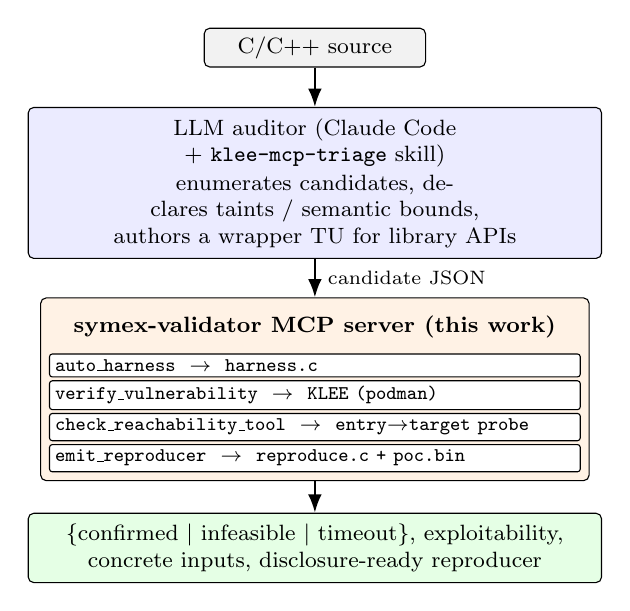
\begin{tikzpicture}[
  font=\footnotesize,
  box/.style={draw, rounded corners=2pt, align=center, inner sep=4pt,
              text width=70mm},
  src/.style ={draw, rounded corners=2pt, align=center, inner sep=3pt,
               fill=gray!10, text width=26mm},
  tool/.style={draw, rounded corners=1pt, align=left, inner sep=2pt,
               fill=white, font=\scriptsize\ttfamily, text width=66mm},
  llm/.style ={box, fill=blue!8},
  result/.style ={box, fill=green!10},
  srvtitle/.style={font=\footnotesize\bfseries, align=center},
  arr/.style ={-Latex, thick},
  node distance=5mm,
]

\node[src] (src) {C/C++ source};

\node[llm, below=5mm of src] (llm) {%
  LLM auditor (Claude Code + \texttt{klee-mcp-triage} skill)\\[1pt]
  enumerates candidates, declares taints / semantic bounds,\\
  authors a wrapper TU for library APIs};

\node[srvtitle, below=6mm of llm] (srvtitle)
  {symex-validator MCP server (this work)};
\node[tool, below=2pt of srvtitle] (t1)
  {auto\_harness \ $\rightarrow$ \ harness.c};
\node[tool, below=1pt of t1] (t2)
  {verify\_vulnerability \ $\rightarrow$ \ KLEE (podman)};
\node[tool, below=1pt of t2] (t3)
  {check\_reachability\_tool \ $\rightarrow$ \ entry$\to$target probe};
\node[tool, below=1pt of t3] (t4)
  {emit\_reproducer \ $\rightarrow$ \ reproduce.c + poc.bin};

\begin{scope}[on background layer]
  \node[draw, rounded corners=2pt, fill=orange!10,
        inner sep=3pt, fit=(srvtitle)(t1)(t2)(t3)(t4)] (srv) {};
\end{scope}

\node[result, below=4mm of srv] (res) {%
  \{confirmed $\mid$ infeasible $\mid$ timeout\}, exploitability,\\
  concrete inputs, disclosure-ready reproducer};

\draw[arr] (src) -- (llm);
\draw[arr] (llm) -- node[right=1pt,font=\scriptsize] {candidate JSON} (srv.north);
\draw[arr] (srv) -- (res);

\end{tikzpicture}
\end{document}
